% Generated by render-figures.mjs from scene.mjs and figures.mjs.
\documentclass[tikz,border=0pt]{standalone}
\usepackage{xcolor}
\definecolor{bg}{HTML}{1B1F27}
\definecolor{fg}{HTML}{E6EDF3}
\definecolor{dim}{HTML}{9AA5B1}
\definecolor{c1}{HTML}{7BC47F}
\definecolor{c2}{HTML}{E5826F}
\definecolor{prediction}{HTML}{6EA8FE}
\definecolor{observed}{HTML}{F0C060}
\definecolor{epipolar}{HTML}{B39DDB}
\begin{document}
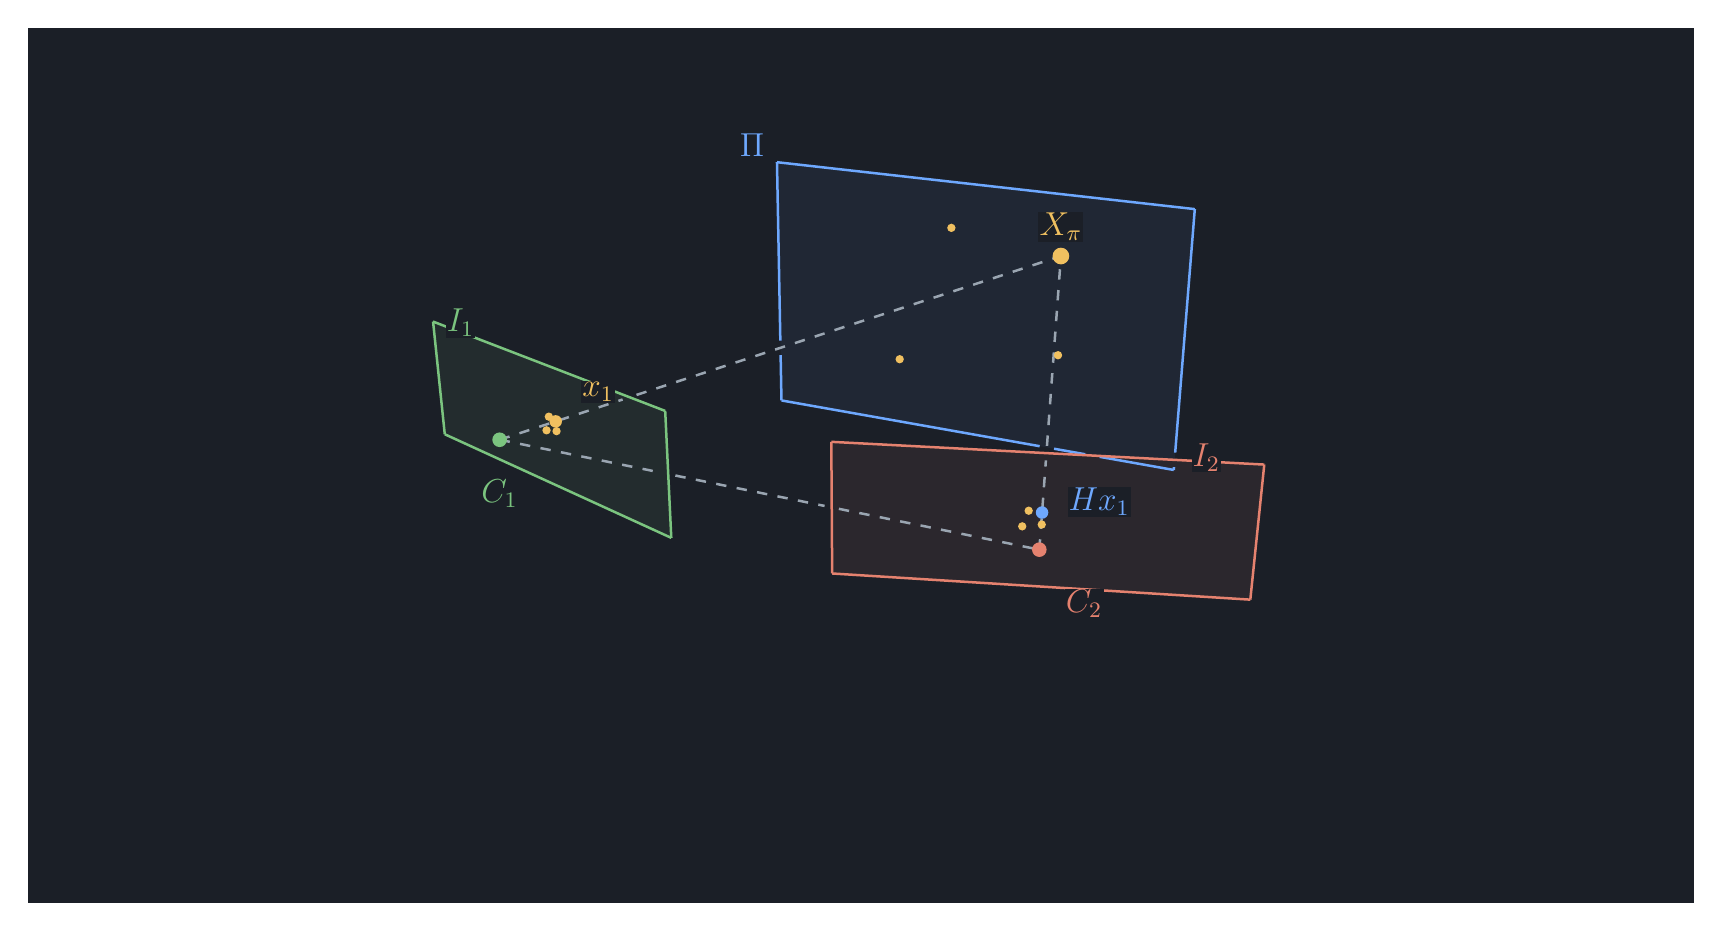
\begin{tikzpicture}[x={(0.026458333cm,0)},y={(0,-0.026458333cm)},every node/.style={font=\fontsize{12}{14}\selectfont}]
\path[use as bounding box] (0,0) rectangle (800,420);
\fill[bg] (0,0) rectangle (800,420);
\path[fill=prediction!6!bg,draw=none,line width=0.0000bp] (361.8133,178.9211) -- (550.1243,212.2904) -- (560.2108,87.0872) -- (359.6587,64.5693) -- cycle;
\path[fill=c1!8!bg,draw=none,line width=0.0000bp] (200.2013,195.1536) -- (308.9273,244.8866) -- (306.0019,183.9573) -- (194.5858,141.0692) -- cycle;
\path[fill=c2!8!bg,draw=none,line width=0.0000bp] (386.1454,261.9824) -- (586.8517,274.5397) -- (593.5570,209.7062) -- (385.7373,198.7860) -- cycle;
\draw[prediction,line width=0.9000bp] (361.8133,178.9211) -- (485.7440,200.8820);
\draw[prediction,line width=0.9000bp] (492.6366,202.1034) -- (507.6394,204.7619);
\draw[prediction,line width=0.9000bp] (514.5320,205.9833) -- (550.1243,212.2904);
\draw[prediction,line width=0.9000bp] (550.1243,212.2904) -- (550.2336,210.9332);
\draw[prediction,line width=0.9000bp] (550.7957,203.9558) -- (560.2108,87.0872);
\draw[prediction,line width=0.9000bp] (560.2108,87.0872) -- (359.6587,64.5693);
\draw[prediction,line width=0.9000bp] (359.6587,64.5693) -- (361.2716,150.1709);
\draw[prediction,line width=0.9000bp] (361.4035,157.1696) -- (361.8133,178.9211);
\draw[c1,line width=0.9000bp] (200.2013,195.1536) -- (308.9273,244.8866);
\draw[c1,line width=0.9000bp] (308.9273,244.8866) -- (306.0019,183.9573);
\draw[c1,line width=0.9000bp] (306.0019,183.9573) -- (194.5858,141.0692);
\draw[c1,line width=0.9000bp] (194.5858,141.0692) -- (200.2013,195.1536);
\draw[c2,line width=0.9000bp] (386.1454,261.9824) -- (586.8517,274.5397);
\draw[c2,line width=0.9000bp] (586.8517,274.5397) -- (593.5570,209.7062);
\draw[c2,line width=0.9000bp] (593.5570,209.7062) -- (385.7373,198.7860);
\draw[c2,line width=0.9000bp] (385.7373,198.7860) -- (386.1454,261.9824);
\draw[dim,line width=0.9000bp,dash pattern=on 3.75bp off 3.75bp] (226.5308,197.7939) -- (304.0278,213.5733);
\draw[dim,line width=0.9000bp,dash pattern=on 3.75bp off 3.75bp] (310.8870,214.9699) -- (382.5108,229.5535);
\draw[dim,line width=0.9000bp,dash pattern=on 3.75bp off 3.75bp] (389.3701,230.9501) -- (485.5812,250.5399);
\draw[dim,line width=0.9000bp,dash pattern=on 3.75bp off 3.75bp] (226.5308,197.7939) -- (285.5816,178.4660);
\draw[dim,line width=0.9000bp,dash pattern=on 3.75bp off 3.75bp] (292.2343,176.2885) -- (495.9515,109.6097);
\draw[dim,line width=0.9000bp,dash pattern=on 3.75bp off 3.75bp] (485.5812,250.5399) -- (488.7334,207.7021);
\draw[dim,line width=0.9000bp,dash pattern=on 3.75bp off 3.75bp] (489.2471,200.7210) -- (495.9515,109.6097);
\fill[c1] (226.5308,197.7939) circle[radius=2.6250bp];
\fill[c2] (485.5812,250.5399) circle[radius=2.6250bp];
\fill[observed] (495.9515,109.6097) circle[radius=3.0000bp];
\fill[observed] (253.4474,188.9838) circle[radius=2.2500bp];
\fill[prediction] (486.8921,232.7247) circle[radius=2.2500bp];
\fill[observed] (418.5547,159.1297) circle[radius=1.5000bp];
\fill[observed] (249.0437,193.2609) circle[radius=1.5000bp];
\fill[observed] (477.3806,239.3560) circle[radius=1.5000bp];
\fill[observed] (494.5532,157.2164) circle[radius=1.5000bp];
\fill[observed] (253.8526,193.6575) circle[radius=1.5000bp];
\fill[observed] (486.7404,238.4826) circle[radius=1.5000bp];
\fill[observed] (443.3663,96.0834) circle[radius=1.5000bp];
\fill[observed] (250.1550,186.7126) circle[radius=1.5000bp];
\fill[observed] (480.4744,231.8550) circle[radius=1.5000bp];
\node[text=prediction,anchor=center,fill=bg,inner sep=0.4bp] at (347.6587,56.5693) {$\Pi$};
\node[text=c1,anchor=center,fill=bg,inner sep=0.4bp] at (207.8138,141.8108) {$I_1$};
\node[text=c1,anchor=center,fill=bg,inner sep=0.4bp] at (226.5308,223.7939) {$C_1$};
\node[text=c2,anchor=center,fill=bg,inner sep=0.4bp] at (565.7741,206.1752) {$I_2$};
\node[text=c2,anchor=west,fill=bg,inner sep=0.4bp] at (497.5812,276.5399) {$C_2$};
\node[text=observed,anchor=center,fill=bg,inner sep=0.4bp] at (495.9515,95.6097) {$X_\pi$};
\node[text=observed,anchor=west,fill=bg,inner sep=0.4bp] at (265.4474,174.9838) {$x_1$};
\node[text=prediction,anchor=west,fill=bg,inner sep=0.4bp] at (498.8921,227.7247) {$Hx_1$};
\end{tikzpicture}
\end{document}
